%% Please do not delete the following line
%% This is the Overleaf LaTeX template for the journal Nuclear Physics A.
%% Copyright 2007-2020 Elsevier Ltd
%% 
%% This file is part of the 'Elsarticle Bundle'.
%% ---------------------------------------------
%% 
%% It may be distributed under the conditions of the LaTeX Project Public
%% License, either version 1.2 of this license or (at your option) any
%% later version.  The latest version of this license is in
%%    http://www.latex-project.org/lppl.txt
%% and version 1.2 or later is part of all distributions of LaTeX
%% version 1999/12/01 or later.
%% 
%% The list of all files belonging to the 'Elsarticle Bundle' is
%% given in the file `manifest.txt`''.
%% 
%% Template article for Elsevier's document class `elsarticle'
%% with harvard style bibliographic references
\documentclass[final,5p,times,twocolumn,authoryear]{elsarticle}
\journal{}  % Leave empty, then the journal name will be printed

% Bold text
\usepackage{bbold}

% Title and section formatting
\usepackage{titlesec}

% Mathematical symbols and fonts
\usepackage{amsmath}
\usepackage{amssymb}
\usepackage{amsfonts}
\usepackage{bm}

% Quantum computing packages
\usepackage{qcircuit}
\usepackage{tikz}
\usepackage{braket}
\usepackage{physics}

% Additional useful packages
\usepackage{hyperref}
\usepackage{cleveref}
\usepackage{mathtools}
\usepackage{caption}
\usepackage{geometry}

% Table packages
\usepackage{booktabs,caption}
\usepackage[flushleft]{threeparttable}
\usepackage{array}

\newcommand*{\Scale}[2][4]{\scalebox{#1}{$#2$}}%

% Remove "Preprint submitted to Elsevier" line
\makeatletter
\def\ps@pprintTitle{%
 \let\@oddhead\@empty
 \let\@evenhead\@empty
 \def\@oddfoot{\footnotesize\itshape
       \hfill\today}%
 \let\@evenfoot\@oddfoot}
\makeatother

% Change the font of subsection to bold and upright
\titleformat{\section}
  {\normalfont\fontsize{12}{15}\bfseries}{\thesubsection}{1em}{}

% Change the font of subsection to bold and upright
\titleformat{\subsection}
  {\normalfont\fontsize{10}{15}\bfseries}{\thesubsection}{1em}{}

% Change the font of subsubsection to italic
\titleformat{\subsubsection}
  {\normalfont\fontsize{9}{15}\itshape \bfseries}{\thesubsubsection}{1em}{}

\begin{document}

\begin{frontmatter}

    \title{Surface code related paper survey}

    \author{Group 28}

    \begin{abstract}
        %% Text of abstract
        Today, Quantum computers have high error rates compared to the classical computer. In order to make quantum computers useful, error rates have to be as low as 1 in a trillion. While a typical transistor in a microprocessor can run for about a billion years at a billion operations per second, without ever suffering a hardware fault due to any form of interference. A huge improvement in performance is needed, since the typical quantum bits become randomized in about one one-thousandth of a second. Classical error correction employ redundacy, however, it is impossible for quantum code due to no-cloning theorem. In this review, we will summarize one of the promising method – surface code. Besides, the novel improvement of the algorithm and decoder will also be provided.
    \end{abstract}

    \begin{keyword}
        %% keywords here, in the form: keyword \sep keyword, up to a maximum of 6 keywords
        Quantum Computation \sep Quantum Error Correction \sep Surface Code \sep Stabilizer codes
    \end{keyword}


\end{frontmatter}

%\tableofcontents

%% \linenumbers

%% main text

\section{Introduction}
\label{introduction}
Quantum computing is a rapidly developing field, and its future is full of exciting possibilities. With breakthroughs from various promising teams, quantum computers are fast approaching the point where they can start to benefit our society. However, in order to fully explore the potential of quantum computers, complex design flows have to be carefully designed and employed to boost the accuracy and efficiency of quantum computing development. Among the different methodologies, error correction is a critical component in ensuring the reliable operation of quantum computers. One of the most prominent error correction schemes is the surface code, which has garnered significant attention due to its robustness and scalability. Surface codes, a class of topological quantum codes, play a vital role in protecting quantum information from decoherence and operational errors. The surface code utilizes a two-dimensional lattice of qubits with stabilizers to detect and correct errors. Recent advancements have focused on improving the efficiency and performance of surface code decoders, stabilizers, and associated algorithms, which are pivotal for practical quantum computing. Generally, implementing and improving surface codes is a complex task. Unlike classical error correction, quantum error correction deals with qubits that exist in superpositions, making the detection and correction of errors more challenging. The design and optimization of decoders and stabilizers, which are responsible for identifying and rectifying errors, are crucial for enhancing the fidelity of quantum computations.

\textbf{to be modified}
In Section II, we provide a comprehensive review of the surface code, including its foundational principles and its importance in quantum error correction. In Section III, we delve into recent improvements in surface code decoders, examining various approaches to enhance their accuracy and efficiency. Section IV discusses advancements in stabilizer codes and their role in the implementation of the surface code. Finally, in Section V, we explore algorithmic developments that leverage the surface code, highlighting their potential impact on the future of quantum computing.

\section{Review of the surface code}
\label{review}
section2

\section{Decoder}
\label{decoder}
As we mentioned in Section 2, decoders are used to perform inference of the error. After the decoder makes a guess of the channel error, the recovery operation can be implemented. However, increasing the accuracy of the decoder usually leads to higher computational complexity, making it slower at making guesses. The trade-off between accuracy and complexity is vital for quantum error correction. In Section 2, we discussed the details of MWPM. Here, we provide a review of a paper that confirms that adapting decoding algorithms to the specific noise characteristics of a quantum device creates more efficient and effective quantum error correction.

\subsection{Tensor-network decoder}

The biggest difference from MWPM is that MWPM only takes Pauli noise into account, and it assumes an uncorrelation between $X$ error and $Z$ error. But, the two-dimensional tensor-network method is provided with the noise map. It can be optimally adapted to arbitrary local noise, including non-Pauli noise, and can also handle correlated noise. The decoding algorithm involves constructing a square-lattice tensor network using information from the syndrome and the suspected noise map, then contracting the network using the time-evolving block decimation (TEBD) algorithm.

\subsubsection{Tensor Network States}

A tensor network can be visualized as a graph where each vertex represents a tensor, a multi-index array of complex numbers. The number of edges incident to a vertex corresponds to the number of tensor indices, with the dimension of an index called the bond dimension. When two vertices are connected by an edge, their corresponding indices are summed over (contracted), similar to matrix multiplication. A vertex can have incident edges not connected to another vertex, called physical indices, which are not contracted.

\subsubsection{Surface Code Wave Function}

The surface code wave function for any encoded state can be described as a projected entangled pair state (PEPS), represented on a square lattice where each tensor corresponds to a physical qubit, which is shown in Figure~\ref{fig:TN_layout}(a). The PEPS structure implies that the density operator can be expressed as a projected entangled pair operator (PEPO).
\subsubsection{Logical Channel Calculation}

For noiseless syndrome extraction, the logical channel $R_s \circ N$ can be calculated by computing all 16 elements of the Pauli transfer matrix: $C_{ij} = {\rm Tr}(L_i(R_s\circ N(L_j)))$
where $L_i$ , $L_j$ are logical Pauli operators, $N$ is noise map. The tensor-network structure preserves the PEPS form during the application of local noise $N$ , recovery  $R_s$, and logical Pauli $L_i$ , allowing  to be expressed as a multi-layer PEPS. Evaluating the trace involves tracing out pairs of physical indices, resulting in a tensor network with no physical indices. This tensor network can be compressed into a single layer by contracting along the time dimension. The resulting square-lattice tensor network can then be contracted using methods like treating the left-hand column as a matrix product state (MPS), evolving it by applying columns sequentially, and using singular value decomposition to control bond dimension growth. Alternatively, the square lattice tensor network can be contracted exactly by merging tensors in the left column into a single tensor, then contracting tensors from the remaining network column by column. The process is shown in the Figure~\ref{fig:TN_layout}.

\begin{figure}[h]
    \centering
    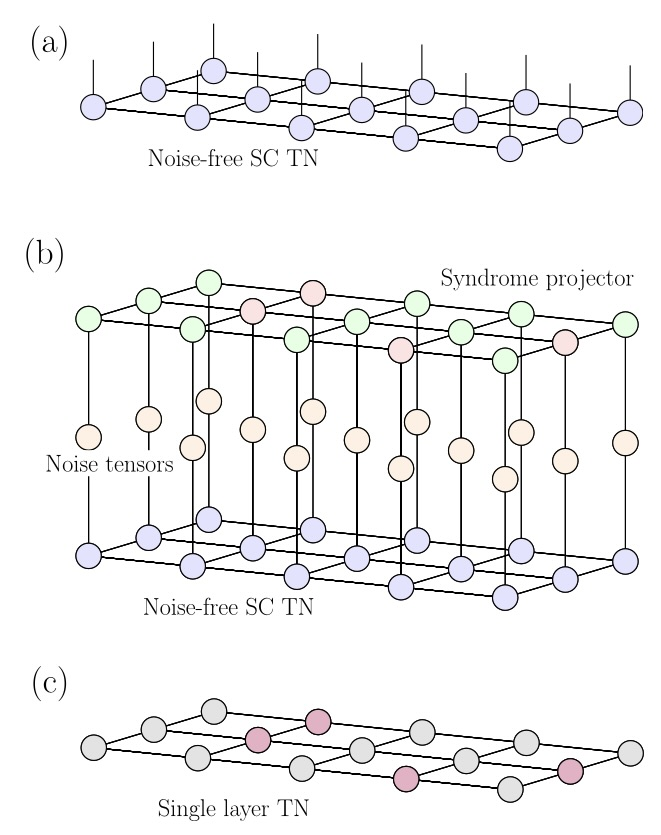
\includegraphics[width=0.4\textwidth]{sections/3_decoder/TN_layout.jpg}
    \caption{(a) A square-lattice PEPS depicting a surface code state, with each tensor having one physical index. (b) A tensor network representing an entry Cij of the Pauli transfer matrix of the logical channel for the surface code under a local noise map with noiseless syndrome extraction. There are three layers corresponding to the noiseless surface code state, local noise, and a syndrome projector, with physical indices traced out. (c) The same tensor network from (b) expressed as a single-layer tensor network which is obtained by vertically contracting the three layers.}
    \label{fig:TN_layout}
\end{figure}

\subsection{Recognizing critical noise parameters using simulation-based decoding}

The paper provides how to identify the most crucial noise in the noise map. If a surface code with a local physical noise map $N$. We can find the optimal decoder that achieves optimal performance for this noise map Then we adjust the miscalibrated decoder, with different parameter $N'$ . If one single noise parameter is different from the optimal parameter, but the result is identical to the optimal one, then we can indicate that the noise is not crucial. The paper have done some adaption about three primary noise features: coherence, inhomogeneity, and bias.
\subsubsection{Coherence}

Quantum noise involves systematic, non-random errors, such as unitary over-rotations due to imperfect gate control. Theoretical analyses of quantum error correcting codes often assume a Pauli noise model, where errors are characterized by random Pauli errors drawn from a probability distribution. This simplifies calculations, especially for stabilizer codes like the surface code, as Pauli noise can be efficiently simulated within the stabilizer formalism. However, physical systems rarely adhere exactly to this assumption. Non-Pauli noise types, such as amplitude damping and systematic over rotations due to imperfect gate control, are common but often overlooked. In order to differentiate from Pauli noise, the author refers to non-Pauli noise as coherent noise. Coherent noise introduces off-diagonal elements in the $\chi$ matrix representation of quantum channels, indicating interactions between different Pauli errors. Previous studies have shown that the surface code's performance can be significantly impacted by coherent noise, sometimes even more so than by Pauli noise. The paper investigates two noise models: single-qubit unitary rotations and systematic over-rotations in CNOT gates. The author compares the performance of different decoders, including an optimal decoder, a decoder considering only incoherent noise components (Pauli' decoder), and a standard minimum-weight perfect matching (MWPM) decoder applied separately to $X$ and $Z$ syndrome data. The paper reveals that adapting the decoder to consider the full noise map, including coherent components, can lead to performance improvements over decoders optimized solely for incoherent noise. However, the magnitude of this improvement is relatively small.

\subsubsection{Inhomogeneity}

Noise in many quantum computing system is spatially inhomogeneous, that is, it varies across different qubits in the device. The paper take noise model of amplitude-phase damping into account. As the \textbf{equation (6)(7)} shows, $\gamma$ represents damping probability and $\lambda$ scattering probabilities. We can assign it as relaxation time $T_1$ and the dephazing time $T_2$ by $e^{-t/T_2}$ = $\sqrt{(1-\gamma)(1-\lambda)}$ and $e^{-t/T_1} = 1 - \gamma$. In experiments, $T_1$ and $T_2$ times can vary significantly over different qubits in a device. The results of our simulations with different decoders are shown in Figure~\ref{fig:T1_fixed}. The first decoder is optimal, which is perfectly fit to the $T_1$ and $T_2$. The second 'uniform' one only have the average of $T_1$ and $T_2$ of each qubit. The third decoder 'ratio' only has information about ratio of $T_1$ and $T_2$ on each qubit. The fourth decoder is simply standard MWPM using a uniformly weighted syndrome graph. The result are clear that the optimal one which equipped with all the information about damping noise outperforms the standard one. The most interesting part is that even just have the ratio of $T_1$ and $T_2$ also improved significantly from the standard one.

\begin{figure}[h]
    \centering
    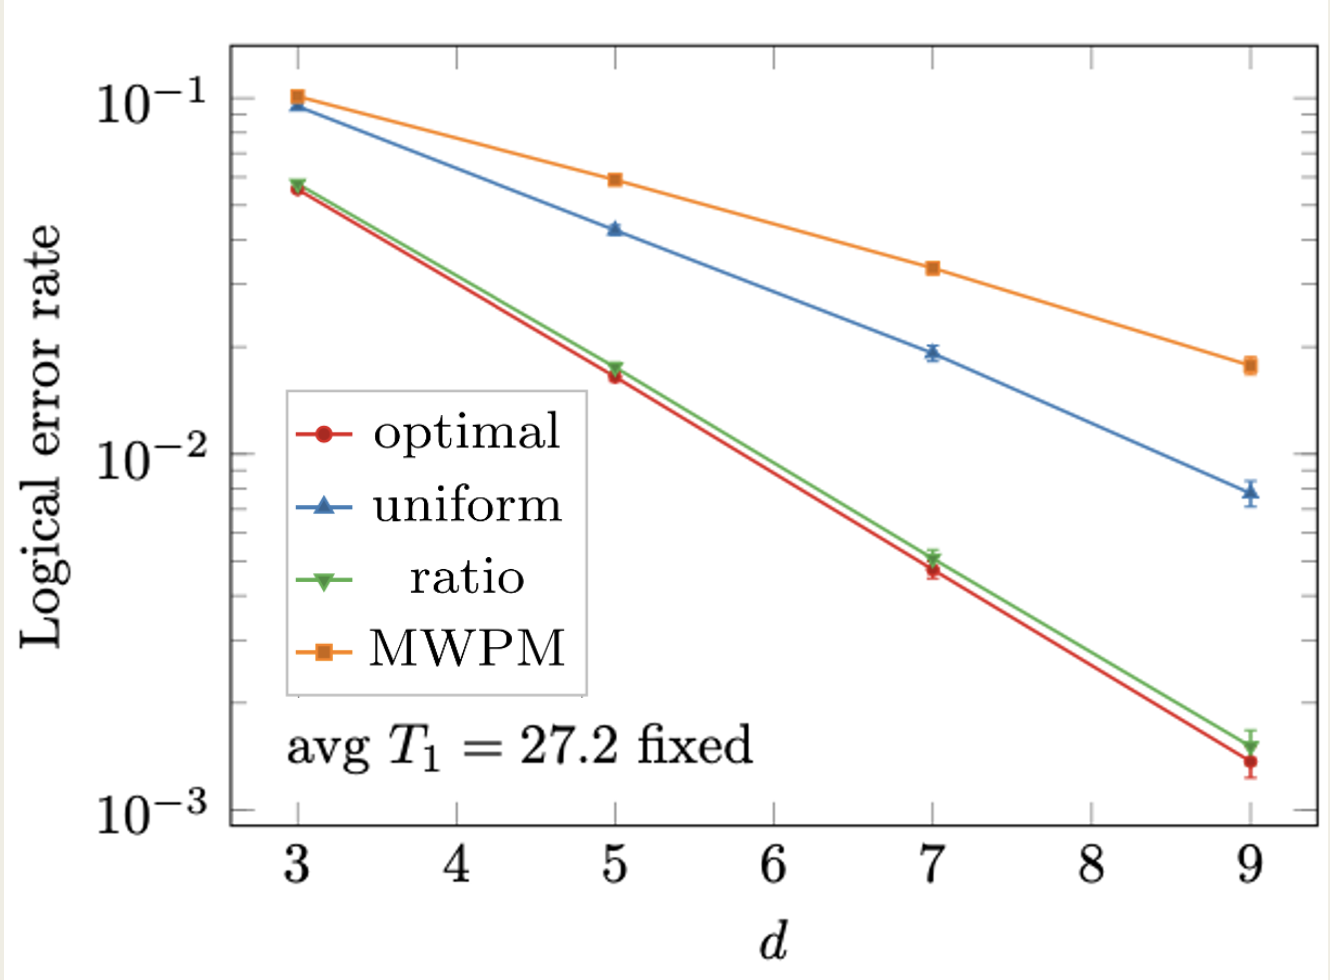
\includegraphics[width=0.4\textwidth]{sections/3_decoder/T1_fixed.png}
    \caption{}
    \label{fig:T1_fixed}
\end{figure}

$$ N_{APD}(\rho) =
    \left(\begin{array}{cc}
            \rho_{00} +  \gamma\rho_{11}          & \rho_{01}\sqrt{(1-\gamma)(1-\lambda)} \\
            \rho_{10}\sqrt{(1-\gamma)(1-\lambda)} & \rho_{11}(1-\gamma)
        \end{array}\right)
$$
$$=
    \left(\begin{array}{cc}
            1-\rho_{11}e^{-t/T_1} & \rho_{01}e^{-t/T_2} \\
            \rho_{01}^*e^{-t/T_2} & \rho_{11}e^{-t/T_1}
        \end{array}\right)
$$


\subsection{Bias}

The paper defines a Pauli noise model as biased when one Pauli error occurs with significantly higher probability than others. As the paragraph aforementioned, we designate either $X$, $Y$, or $Z$ as the dominant error, and the surface code's performance heavily relies on the local basis used for defining checks. The author focus is on single-qubit $Y$-biased Pauli noise, where $p_X$ = $p_Z$ , $p := p_X +p_Y +p_Z$, and $\eta := \frac{p_Y}{p_X + p_Z}$ . The simulation results, depicted in Figure~\ref{fig:eta}, illustrate the effects of depolarizing (unbiased) noise corresponding to $\eta$ = 0.5 and biased noise with $\eta$ = 100. For depolarizing noise, as shown in Figure~\ref{fig:eta}(a), the miscalibrated decoder achieves nearly same logical error rates compared to the optimal decoder, with the threshold barely altering. On the other hand, under biased noise with fixed $\eta = 100$, as shown in Figure~\ref{fig:eta}(b), there is a significant difference observed between the two decoders. The logical error rate for the largest system size with the miscalibrated decoder. These findings suggest that sensitivity to decoder miscalibration escalates with noise bias. Notably, the decoder needs a number of information about the bias $\eta$ to perform optimally
\begin{figure}[h]
    \centering
    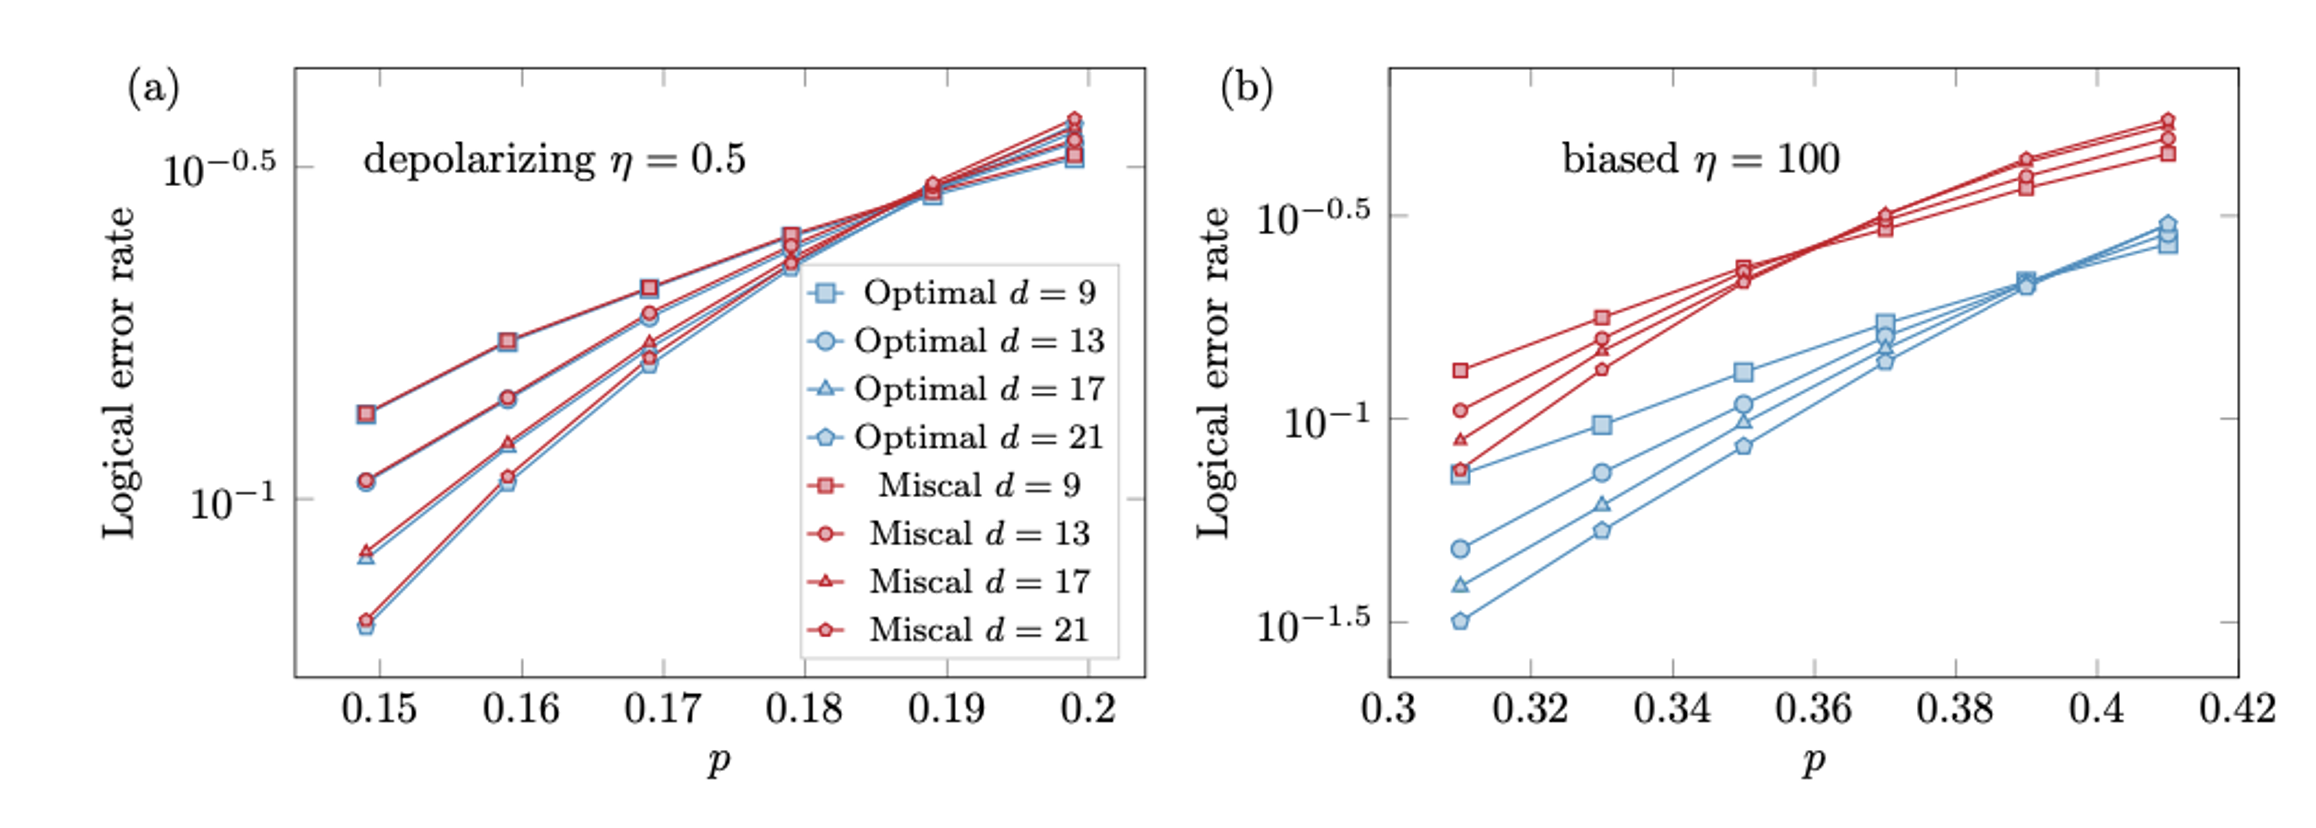
\includegraphics[width=0.5\textwidth]{sections/3_decoder/eta.png}
    \caption{The effect of noise bias on surface-code decoding. 'Optimal' means that the noise model input to the decoder is exactly the physical noise model, and 'Miscal' means that the average infidelity in the decoder noise model is mischaracterized pdec = p/2. (a) physical noise model is depolarizing noise, while in (b) it is biased noise with $\eta$ = 100}
    \label{fig:eta}
\end{figure}

By focusing on coherence, inhomogeneity, and bias, and understanding their impact on decoder performance, the paper provides a framework for optimizing surface-code decoders by leveraging detailed noise information. This targeted approach not only aids in developing better decoders but also informs the design of noise characterization techniques, ensuring that future quantum computing systems can maintain high levels of fault tolerance with reduced overhead.

\section{Stabilizer}
\label{stabilizer}
Stabilizers are used to detect errors in the quantum state. In the context of surface code, stabilizers are operators that measure a group of qubits. When an error occurs, it changes the measurement outcomes of these stabilizers, indicating the presence and type of error. Nonetheless, as quantum computing scales, the defects in qubits and couplers due to fabrication errors become inevitable. These can significantly disrupt the surface codes error-correcting capabilities, which are essential for reliable quantum computation. \textbf{The paper (Low-Overhead Defect-Adaptive Surface Code with Bandage-Like Super-Stabilizers)} propose an automated adapter for surface codes that can handle defective lattices. This adapter includes three main subroutines: boundary deformation, internal defect disabling, and stabilizer patching. In this sector, we will briefly go through all the steps.

\subsection{Constructing stabilizer steps}
\subsubsection{Boundary deformation}

\begin{figure*}[h]
    \centering
    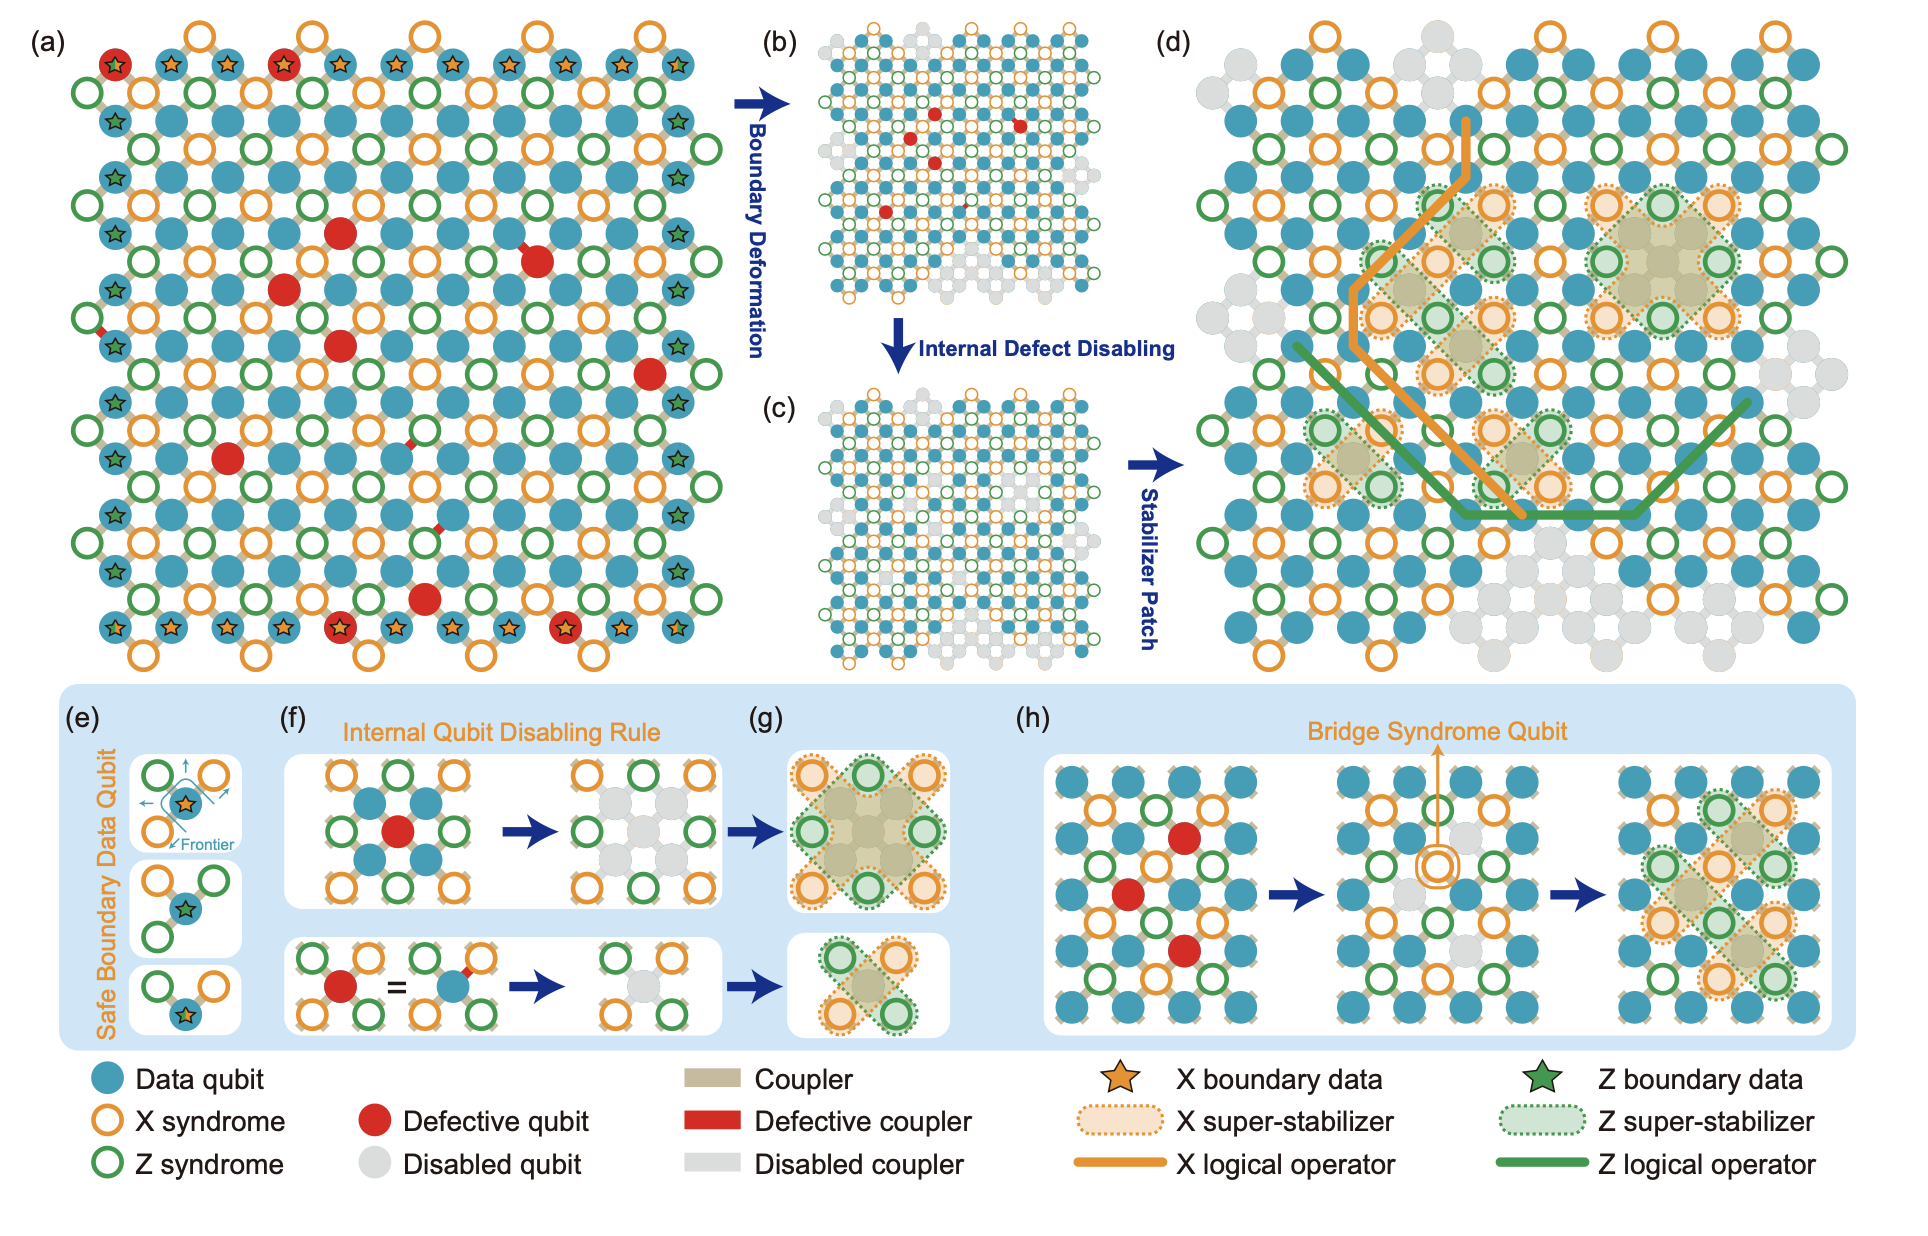
\includegraphics[width=0.8\textwidth]{sections/4_stabilizer/Fig1.png}
    \caption{The Construction Steps for the Defect-Adaptive Surface Code.(a) An instance of a defective surface code lattice,the defective qubits and couplers in red, and boundary qubits are marked with star symbols. (b) code lattice after boundary deformation (c) code lattice after internal defect disabling. (d) code lattice after stabilizer patch, respectively. (e) The depiction for boundary data qubits and their frontiers, including X, Z, and corner boundary data qubits from top to bottom, along with their frontiers, encompassing couplers and syndrome qubits around data qubits. (f) Depicts the rules for internal defect disabling, showcasing the disabled qubits rules for defect syndrome qubits, data qubits, and couplers from top to bottom. (g) practice traditional super-stabilizers if internal defect qubits are not clustered. (h) in clustered situations, these super-stabilizers can stretch across weight-1 and bridge syndrome qubits. The middle of (h) highlights a bridge syndrome qubit for illustration purposes.}
    \label{fig:Fig1}
\end{figure*}

We first begin the boundary deformation process by addressing defects along the boundary, focusing on removing unsafe boundary data qubits and redundant syndrome qubits. A boundary data qubit is considered safe if it meets three conditions: the qubit itself is defect-free, its surrounding frontier—including neighboring syndrome qubits and couplers—is also defect-free, and this frontier aligns with the boundary type, as example in Figure~\ref{fig:Fig1}(e). We can simply use a Breadth-First Search (BFS) algorithm to evaluate the safety of each boundary data qubit. If one unsafe data qubit is found, the surrounding redundant syndrome qubits—those that are defective, have no undisabled data qubit neighbors, or are of different types from the boundary—are disabled. Following these guidelines, the surface code in Figure~\ref{fig:Fig1}(a), will turn into Figure~\ref{fig:Fig1}(b). The BFS algorithm continues to reevaluate boundary data qubits, checking any new unsafe ones and redundant syndrome qubits, until no new unsafe boundary data qubits are detected. This iterative process results in a defect-free boundary.




\subsubsection{Internal defect disabling}

The process of internal defect disabling involves addressing defects within the lattice. Internal defects are classified into three types: data qubits, syndrome qubits, and couplers. According to the rules, for data qubit and coupler defects, we disable the corresponding data qubits, while for syndrome qubit defects, we disable the syndrome qubits and their neighboring data qubits, which shown in Figure~\ref{fig:Fig1(f)}. This is because internal data qubits need two X and two Z syndrome qubits to detect Z and X errors. The defects must be addressed in a specific order—first defective syndrome qubits, then defective data qubits, and finally defective couplers—in order to ensure each rule is applied only once and to prevent conflicts. Additionally, we disable weight-0 syndrome qubits (a weight-n syndrome qubit has n undisabled data qubit neighbors) resulting from these actions. Internal defects may cluster, particularly at high defect rates, leading to situations like weight-1 syndrome qubits and bridge syndrome qubits, where a syndrome qubit connects to two active data qubits along the same diagonal. As shown in Figure~\ref{fig:Fig1}(h). Disabling these types of syndrome qubits, doing so might require reapplying internal defect rules, potentially disrupting the boundary shape and causing an avalanche effect where many qubits are disabled. To avoid this, the proposed method do not disable internal weight-1 and bridge syndrome qubits. Instead, the author use a bandage-like super-stabilizer strategy to reduce the number of disabled qubits, minimize super-stabilizer weight, and prevent an avalanche effect. 

\subsubsection{Stabilizer patching}

The proposed bandage-like super-stabilizers connect the same type of gauge syndrome qubits through disabled qubits, covering all internal disabled qubits. For unclustered internal defect qubits, these super-stabilizers are similarly to traditional super-stabilizers, which shown in Figure~\ref{fig:Fig1}(g). While for clustered defect qubits, they stretch across weight-1 and bridge syndrome qubits, preserving more data qubits and maintaining integrity, as  shown in Figure~\ref{fig:Fig1}(g). And then logical operators (X and Z) are placed on paths containing opposing types of syndrome qubits to avoid intersecting super-stabilizers and introducing gauge qubits. Eventually, the proposed method adapts the defect lattice depicted in Figure~\ref{fig:Fig1}(a) into surface code shown in Figure~\ref{fig:Fig1}(d)

\begin{figure}[h]
    \centering
    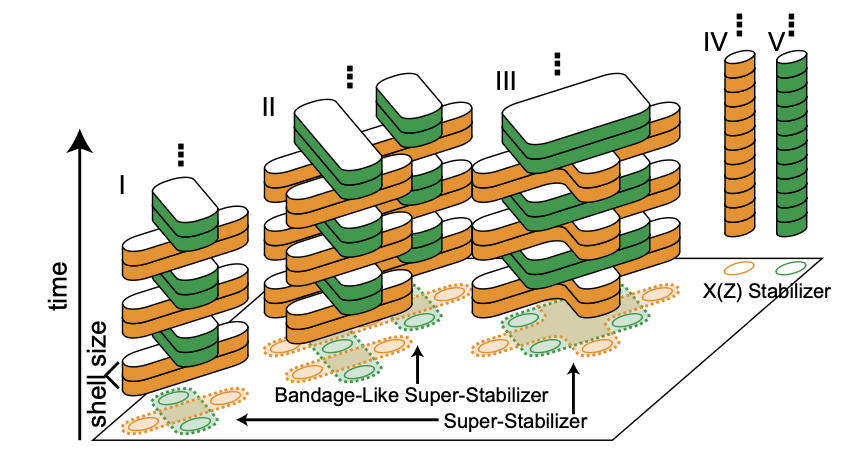
\includegraphics[width=0.4\textwidth]{sections/4_stabilizer/Fig2.png}
    \caption{}
    \label{fig:Fig2}
\end{figure}

\subsection{Stabilizer measurement circuit} 

Due to their anti-commuting gauge operators, constructing the stabilizer measurement circuits for adapted devices can't be directly measured like regular single-syndrome stabilizer. In the method, multiple bandage-like super-stabilizers may combine to form a group of super-stabilizers such as that in Figure~\ref{fig:Fig2}, where a group with two X and two Z bandage-like super-stabilizers. It is essential to ensure that X and Z super-stabilizers in the same group are not measured in the same cycle, while the same type within a group is measured simultaneously.
To enhance error correction capability, the method repeat the measurement of the same type of gauge operator for several consecutive cycles to gather information about each operator's value. The number of consecutive measurement cycles is referred to as the shell size, as shown in Figure~\ref{fig:Fig2}. It is necessary to determine the appropriate shell size for each stabilizer group while considering experimental constraints. There are two strategies for determining the shell size: the global strategy applies the same shell size to all stabilizer groups, while the local strategy assigns each group its own shell size. The choice of shell size depends on the processor and physical system characteristics.

\begin{figure}[h]
    \centering
    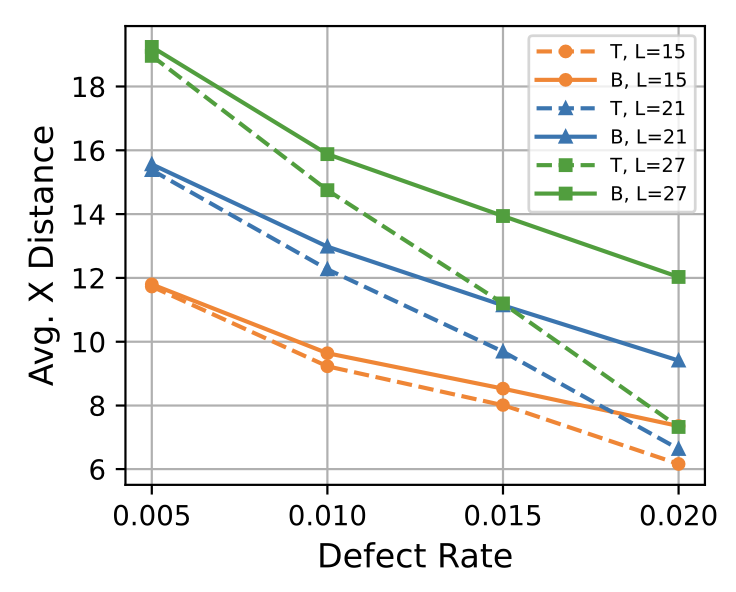
\includegraphics[width=0.3\textwidth]{sections/4_stabilizer/Fig3c.png}
    \caption{Average X Distance vs Defect Rate}
    \label{fig:Fig3c}
\end{figure}

\begin{figure}[h]
    \centering
    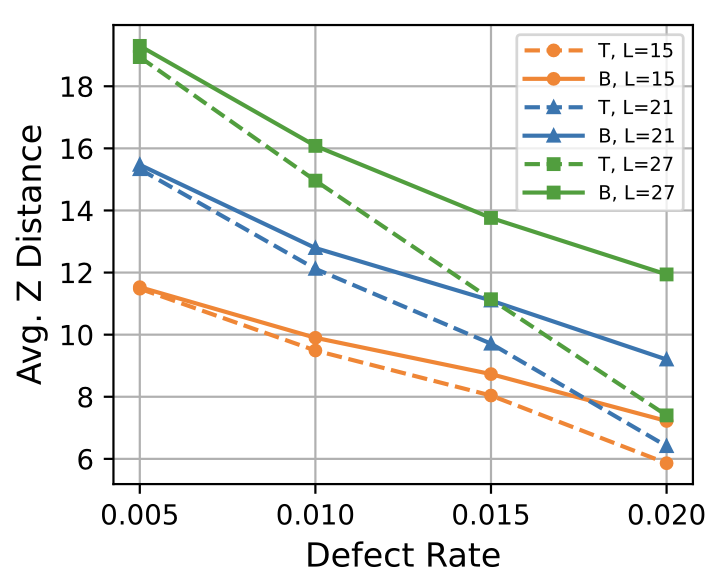
\includegraphics[width=0.3\textwidth]{sections/4_stabilizer/Fig3d.png}
    \caption{Average Z Distance vs Defect Rate}
    \label{fig:Fig3d}
\end{figure}

\begin{figure}[h]
    \centering
    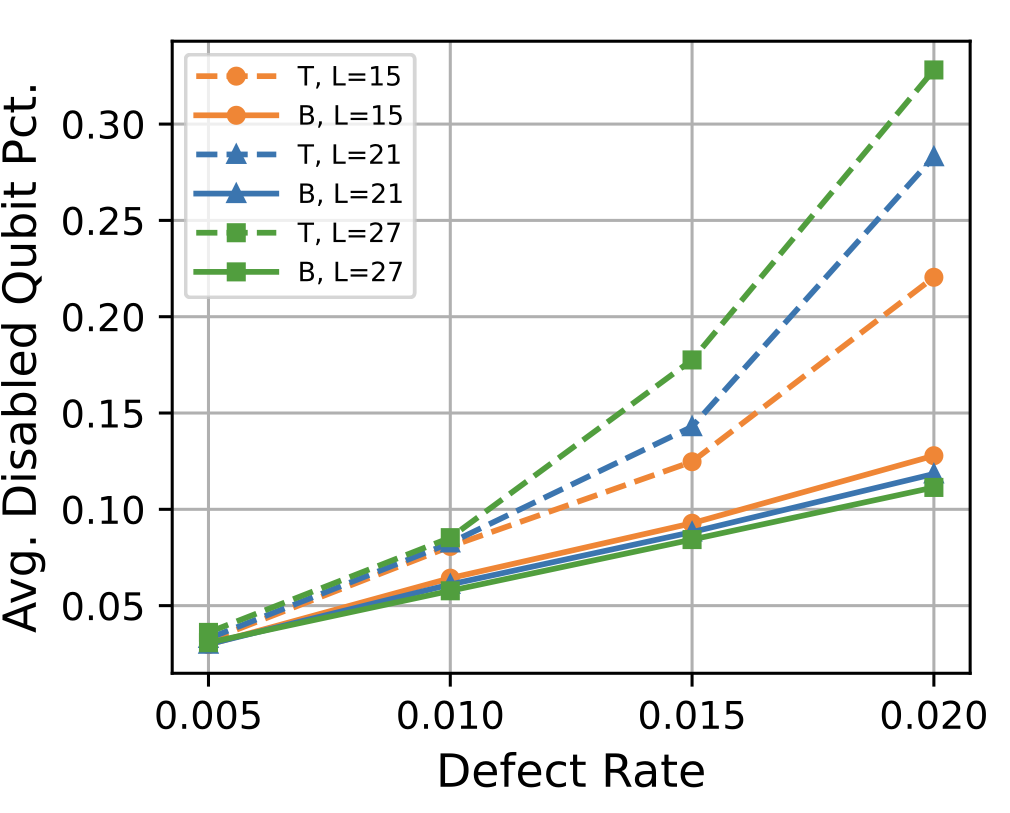
\includegraphics[width=0.3\textwidth]{sections/4_stabilizer/Fig3e.png}
    \caption{Average Z Distance vs Defect Rate}
    \label{fig:Fig3e}
\end{figure}

\subsection{Conclusion}
By following these steps, the method ensures a defect-adaptive surface code with enhanced efficiency, and also avoid overhead. The paper compared the traditional stabilizer with their proposed method. Naturally, code distance will decrease as defect rates gets higher. In contrast to the traditional stabilizer, the bandage stabilizer maintains a superior code distance, and this advantage grows as defect rates increase, similar to the above specific case. The result is demonstrated in Figure~\ref{fig:Fig3c} and Figure~\ref{fig:Fig3d}. Besides, the proposed method also preserves code distance by disabling fewer qubits. The illustration is in Figure~\ref{fig:Fig3e} which shows the average percentage of disabled qubits after adaptation. Despite that disabled qubits increase with defect rates, the proposed method demonstrates a slower increase, which indicate better qubit preservation compared to the traditional method.

\section{Algorithm developments}
\label{algorithm}
section5

%% If you have bibdatabase file and want bibtex to generate the
%% bibitems, please use
%%
\bibliographystyle{elsarticle-harv}
\bibliography{example}

%% else use the following coding to input the bibitems directly in the
%% TeX file.

%%\begin{thebibliography}{00}

%% \bibitem[Author(year)]{label}
%% For example:

%% \bibitem[Aladro et al.(2015)]{Aladro15} Aladro, R., Martín, S., Riquelme, D., et al. 2015, \aas, 579, A101


%%\end{thebibliography}

\end{document}

\endinput
%%
%% End of file `elsarticle-template-harv.tex'.
